\let\negmedspace\undefined
\let\negthickspace\undefined
\documentclass[a4paper,10pt]{article}
\usepackage[a5paper, margin=10mm, onecolumn]{geometry}

\usepackage{tfrupee}
\setlength{\headheight}{1cm}
\setlength{\headsep}{0mm}

\usepackage{gvv-book}
\usepackage{cite}
\usepackage{amsmath,amssymb,amsfonts,amsthm}
\usepackage{gvv}
\usepackage{algorithmic}
\usepackage{graphicx}
\usepackage{textcomp}
\usepackage{xcolor}
\usepackage{txfonts}
\usepackage{listings}
\usepackage{enumitem}
\usepackage{mathtools}
\usepackage{gensymb}
\usepackage{comment}
\usepackage[breaklinks=true]{hyperref}
\usepackage{tkz-euclide} 
\usepackage{listings}                                     
\def\inputGnumericTable{}                                 
\usepackage[latin1]{inputenc}                              
\usepackage{color}                                         
\usepackage{array}                                         
\usepackage{longtable}                                     
\usepackage{calc}                                          
\usepackage{multirow}                                      
\usepackage{hhline}                                        
\usepackage{ifthen}                                        
\usepackage{lscape}


\graphicspath{{./figs/}}


\title{XE:ENGINEERING SCIENCES}

\author{EE25BTECH11051- Shreyas Goud Burra}

\date{}



\begin{document}

\maketitle

\section*{GA: General Aptitude (Compulsory)}
\begin{enumerate}
\item The question below consists of a pair of related words followed by four pairs of words. Select the pair that best expresses the relation in the original pair. \\
Unemployed : Worker
\hfill{\brak{\text{GATE XE 2010}}}

\begin{multicols}{2}
\begin{enumerate}
\item fallow : land
\item unaware : sleeper
\item wit : jester
\item renovated : house
\end{enumerate}
\end{multicols}

\item Choose the most appropriate word from the options given below to complete the following sentence: \\
His rather casual remarks on politics \underline{\hspace{2cm}} his lack of seriousness about the subject.
\hfill{\brak{\text{GATE XE 2010}}}

\begin{multicols}{4}
\begin{enumerate}
\item masked
\item belied
\item betrayed
\item suppressed
\end{enumerate}
\end{multicols}

\item Which of the following options is the closest in meaning to the word below: \\
Circuitous
\hfill{\brak{\text{GATE XE 2010}}}

\begin{multicols}{4}
\begin{enumerate}
\item cyclic
\item indirect
\item confusing
\item crooked
\end{enumerate}
\end{multicols}

\item 25 persons are in a room. 15 of them play hockey, 17 of them play football and 10 of them play both hockey and football. Then the number of persons playing neither hockey nor football is:
\hfill{\brak{\text{GATE XE 2010}}}

\begin{multicols}{4}
\begin{enumerate}
\item 2
\item 17
\item 13
\item 3
\end{enumerate}
\end{multicols}

\item Choose the most appropriate word from the options given below to complete the following sentence: \\
If we manage to \underline{\hspace{2cm}} our natural resources, we would leave a better planet for our children.
\hfill{\brak{\text{GATE XE 2010}}}

\begin{multicols}{4}
\begin{enumerate}
\item uphold
\item restrain
\item cherish
\item conserve
\end{enumerate}
\end{multicols}

\item 5 skilled workers can build a wall in 20 days; 8 semi-skilled workers can build a wall in 25 days; 10 unskilled workers can build a wall in 30 days. If a team has 2 skilled, 6 semi-skilled and 5 unskilled workers, how long will it take to build the wall?
\hfill{\brak{\text{GATE XE 2010}}}

\begin{multicols}{4}
\begin{enumerate}
\item 20 days
\item 18 days
\item 16 days
\item 15 days
\end{enumerate}
\end{multicols}

\item Given digits 2, 2, 3, 3, 3, 4, 4, 4, 4 how many distinct 4 digit numbers greater than 3000 can be formed?
\hfill{\brak{\text{GATE XE 2010}}}

\begin{multicols}{4}
\begin{enumerate}
\item 50
\item 51
\item 52
\item 54
\end{enumerate}
\end{multicols}

\item If $137 + 276 = 435$ how much is $731 + 672$?
\hfill{\brak{\text{GATE XE 2010}}}

\begin{multicols}{4}
\begin{enumerate}
\item 534
\item 1403
\item 1623
\item 1513
\end{enumerate}
\end{multicols}

\item Hari \brak{H}, Gita \brak{G}, Irfan \brak{I} and Saira \brak{S} are siblings \brak{\text{i.e. brothers and sisters}}. All were born on 1\textsuperscript{st} January. The age difference between any two successive siblings \brak{\text{that is born one after another}} is less than 3 years. Given the following facts: \\
i. Hari's age + Gita's age $>$ Irfan's age + Saira's age. \\
ii. The age difference between Gita and Saira is 1 year. However, Gita is not the oldest and Saira is not the youngest. \\
iii. There are no twins. \\
In what order were they born \brak{\text{oldest first}}?
\hfill{\brak{\text{GATE XE 2010}}}

\begin{multicols}{4}
\begin{enumerate}
\item HSIG
\item SGHI
\item IGSH
\item IHSG
\end{enumerate}
\end{multicols}

\item Modern warfare has changed from large scale clashes of armies to suppression of civilian populations. Chemical agents that do their work silently appear to be suited to such warfare; and regretfully, there exist people in military establishments who think that chemical agents are useful tools for their cause. \\
Which of the following statements best sums up the meaning of the above passage:
\hfill{\brak{\text{GATE XE 2010}}}

\begin{enumerate}
\item Modern warfare has resulted in civil strife.
\item Chemical agents are useful in modern warfare.
\item Use of chemical agents in warfare would be undesirable.
\item People in military establishments like to use chemical agents in war.
\end{enumerate}
\end{enumerate}

\section*{A : ENGINEERING MATHEMATICS (Compulsory)}
\begin{enumerate}
\item If $P = \myvec{1 & 1 \\ 1 & 1}$, then $P^8 - 2P^7 + 2P^6 - 4P^5 + 3P^4 - 6P^3 + 2P^2$ equals
\hfill{\brak{\text{GATE XE 2010}}}

\begin{multicols}{4}
\begin{enumerate}
\item P
\item 2P
\item 3P
\item 4P
\end{enumerate}
\end{multicols}

\item Which one of the following matrices has the same eigen values as that of $\myvec{1 & 2 \\ 4 & 3}$?
\hfill{\brak{\text{GATE XE 2010}}}

\begin{multicols}{2}
\begin{enumerate}
\item $\myvec{3 & 4 \\ 1 & 2}$
\item $\myvec{1 & 4 \\ 2 & 3}$
\item $\myvec{4 & 2 \\ 1 & 3}$
\item $\myvec{2 & 4 \\ 1 & 3}$
\end{enumerate}
\end{multicols}

\item The integral $\int_{-1}^{1} x^{-2/3} dx$ is
\hfill{\brak{\text{GATE XE 2010}}}

\begin{enumerate}
\item an improper integral converging to -6.
\item an improper integral converging to 0.
\item not an improper integral but has value -6.
\item a divergent improper integral.
\end{enumerate}

\item The residue of the function $f(z) = \frac{\sin^4 z}{\brak{z+\pi/4}^3}$ at $z = -\pi/4$ is
\hfill{\brak{\text{GATE XE 2010}}}

\begin{multicols}{4}
\begin{enumerate}
\item 2
\item 1
\item -1
\item -2
\end{enumerate}
\end{multicols}

\item The variance of the number of heads resulting from ten independent tosses of a fair coin is
\hfill{\brak{\text{GATE XE 2010}}}

\begin{multicols}{4}
\begin{enumerate}
\item $5/4$
\item $5/2$
\item $3/4$
\item $3/2$
\end{enumerate}
\end{multicols}

\item If the quadrature rule $\int_{0}^{3} f(x)dx = \alpha f(1) + \beta f(3)$ is exact for all polynomials of degree 2 or less, then
\hfill{\brak{\text{GATE XE 2010}}}

\begin{multicols}{2}
\begin{enumerate}
\item $\alpha = 3/4$, $\beta = 3/4$
\item $\alpha = 3/4$, $\beta = 9/4$
\item $\alpha = 9/4$, $\beta = 3/4$
\item $\alpha = 9/4$, $\beta = 9/4$
\end{enumerate}
\end{multicols}

\item Given that $\frac{dy}{dx} = 1+y^2$, $y(0) = 0$, which one of the following is nearest to $y(0.4)$ computed by Euler's method with step size of 0.2 ?
\hfill{\brak{\text{GATE XE 2010}}}

\begin{multicols}{4}
\begin{enumerate}
\item 0.408
\item 0.404
\item 0.208
\item 0.204
\end{enumerate}
\end{multicols}

\item Let $f(x) = \begin{cases} \frac{\sin x}{x} & \text{if } x \neq 0 \\ 1 & \text{if } x = 0 \end{cases}$. Then
\hfill{\brak{\text{GATE XE 2010}}}

\begin{enumerate}
\item f is not continuous at $x=0$.
\item f is continuous at $x=0$ but not differentiable at $x=0$.
\item f is differentiable at $x=0$ and $f'(0)=0$.
\item f is differentiable at $x=0$ and $f'(0)=1$.
\end{enumerate}

\item Let $u(x, y) = \tan{xy(x + y)}$. Then
\hfill{\brak{\text{GATE XE 2010}}}

\begin{enumerate}
\item $x \frac{\partial u}{\partial x} + y \frac{\partial u}{\partial y} = \frac{1}{3}xy(x+y) \sec^2{xy(x + y)}$.
\item $x \frac{\partial u}{\partial x} - y \frac{\partial u}{\partial y} = \frac{1}{3}xy(x+y) \sec^2{xy(x + y)}$.
\item $x \frac{\partial u}{\partial x} + y \frac{\partial u}{\partial y} = 3xy(x + y) \sec^2{xy(x+y)}$.
\item $x \frac{\partial u}{\partial x} - y \frac{\partial u}{\partial y} = 3xy(x+y) \sec^2{xy(x + y)}$.
\end{enumerate}

\item Which one of the following is a particular solution of the ordinary differential equation $\frac{d^2 y}{dx^2} - \frac{dy}{dx} = 2x^2 f(x)$?
\hfill{\brak{\text{GATE XE 2010}}}

\begin{multicols}{2}
\begin{enumerate}
\item $x^2 \int x f(x)dx + \int x^3 f(x)dx$
\item $x^2 \int f(x)dx + \int x^2 f(x)dx$
\item $x^2 \int x f(x)dx - \int x^3 f(x)dx$
\item $x^2 \int f(x)dx - \int x^2 f(x)dx$
\end{enumerate}
\end{multicols}

\item Which one of the following is a possible solution to the partial differential equation $\frac{\partial^2 u}{\partial t^2} - \frac{\partial^2 u}{\partial x^2} = 0$ with boundary conditions $u(0,t)=0, \frac{\partial u(\pi,t)}{\partial x}=0, \text{ for } t \geq 0, u(x,0)=0, \frac{\partial u(x,0)}{\partial t}=\pi, \text{ for } 0 \leq x \leq \pi$?
\hfill{\brak{\text{GATE XE 2010}}}

\begin{enumerate}
\item $u(x,t) = \sum_{n=0}^{\infty} a_n \sin\brak{(n+\frac{1}{2})t} \sin\brak{(n+\frac{1}{2})x}$
\item $u(x,t) = \sum_{n=0}^{\infty} a_n \cos\brak{(n+\frac{1}{2})t} \sin\brak{(n+\frac{1}{2})x}$
\item $u(x,t) = \sum_{n=0}^{\infty} a_n \sin\brak{(n+\frac{1}{2})t} \cos\brak{(n+\frac{1}{2})x}$
\item $u(x,t) = \sum_{n=0}^{\infty} a_n \cos\brak{(n+\frac{1}{2})t} \cos\brak{(n+\frac{1}{2})x}$
\end{enumerate}
\end{enumerate}

\section*{B: FLUID MECHANICS}
\begin{enumerate}
\item A cylindrical container is filled with a liquid up to half of its height. The container is mounted on the centre of a turn-table and is held fixed using a spindle. The turn-table is now rotated about its central axis with a certain angular velocity. After some time interval, the fluid attains rigid body rotation. Which of the following profiles best represents the constant pressure surfaces in the container?
\hfill{\brak{\text{GATE XE 2010}}} \\

\begin{multicols}{2}
\begin{enumerate}
\item \begin{figure}[H]
    \centering
    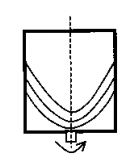
\includegraphics[width=0.4\columnwidth]{B1opt1.png}
    \caption*{}
    \label{fig:opt1}
\end{figure}
\item \begin{figure}[H]
    \centering
    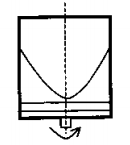
\includegraphics[width=0.4\columnwidth]{B1opt2.png}
    \caption*{}
    \label{fig:opt2}
\end{figure}
\item \begin{figure}[H]
    \centering
    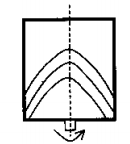
\includegraphics[width=0.4\columnwidth]{B1opt3.png}
    \caption*{}
    \label{fig:opt3}
\end{figure}
\item \begin{figure}[H]
    \centering
    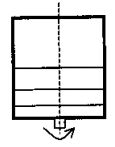
\includegraphics[width=0.4\columnwidth]{B1opt4.png}
    \caption*{}
    \label{fig:opt4}
\end{figure}
\end{enumerate}
\end{multicols}

\item Match the items given in the following two columns using appropriate combinations:
\begin{table}[H]
\centering
\begin{tabular}{ll}
\textbf{Column 1} & \textbf{Column 2} \\
P Ratio of inertial force to viscous force & 1. Reynolds number \brak{\text{Re}} \\
Q Ratio of momentum diffusivity to thermal diffusivity & 2. Froude number \brak{\text{Fr}} \\
R Ratio of inertial force to compressibility force & 3. Prandtl number \brak{\text{Pr}} \\
S Ratio of inertial force to gravity force & 4. Mach number \brak{\text{Ma}} \\
\end{tabular}
\caption*{}
\label{tab:q2}
\end{table}
\hfill{\brak{\text{GATE XE 2010}}}

\begin{multicols}{2}
\begin{enumerate}
\item P-1; R-2; Q-3; S-4
\item P-1; Q-2; R-3; S-4
\item P-1; R-2; S-3; Q-4
\item P-1; S-2; Q-3; R-4
\end{enumerate}
\end{multicols}

\item In the context of boundary layers, which one of the following statements is FALSE ?
\hfill{\brak{\text{GATE XE 2010}}}

\begin{enumerate}
\item It is a frictional layer, close to the body
\item It is a region where the fluid flow is irrotational
\item It is a region across which the pressure gradient is negligible
\item It is a diffusion layer of vorticity
\end{enumerate}

\item Consider an ideal fluid flow past a circular cylinder shown in the figure below. The peripheral velocity at a point P on the surface of the cylinder is
\begin{figure}[H]
    \centering
    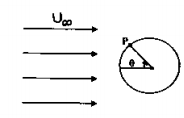
\includegraphics[width=0.4\columnwidth]{Bq4.png}
    \caption*{}
    \label{fig:q4}
\end{figure}
\hfill{\brak{\text{GATE XE 2010}}}

\begin{multicols}{4}
\begin{enumerate}
\item 0
\item $U_\infty$
\item $U_\infty \sin \theta$
\item $2 U_\infty \sin \theta$
\end{enumerate}
\end{multicols}

\item The Rheological diagram depicting the relation between shear stress and strain rate for different types of fluids is shown in the figure below.
\begin{figure}[H]
    \centering
    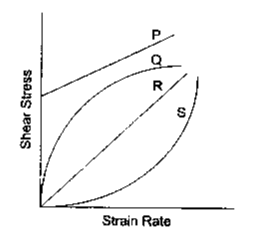
\includegraphics[width=0.4\columnwidth]{Bq5.png}
    \caption*{}
    \label{fig:q5}
\end{figure}
The most suitable relation for flow of tooth paste being squeezed out of the tube is given by the curve
\hfill{\brak{\text{GATE XE 2010}}}

\begin{multicols}{4}
\begin{enumerate}
\item P
\item Q
\item R
\item S
\end{enumerate}
\end{multicols}

\item The diverging limb of a venturimeter is kept longer than the converging limb to
\hfill{\brak{\text{GATE XE 2010}}}

\begin{enumerate}
\item ensure that the flow remains laminar
\item avoid separation
\item ensure that the flow remains turbulent
\item avoid formation of boundary layer
\end{enumerate}

\item The length scale of a model is kept as 1 : 64. The prototype fluid is water. Viscous and gravity forces are equally dominant in the prototype. The required kinematic viscosity \brak{\text{m$^2$/s}} of the fluid used in the model is
\hfill{\brak{\text{GATE XE 2010}}}

\begin{multicols}{2}
\begin{enumerate}
\item 0.100E-07
\item 0.195E-08
\item 0.156E-07
\item 0.125E-07
\end{enumerate}
\end{multicols}

\item Let $\phi$ and $\psi$ represent, respectively, the velocity potential and stream function of a flow field of an incompressible fluid. Which of the following statements are TRUE? \\
P: $\phi$ exists for irrotational flows only \\
Q: $\psi$ exists for both irrotational and rotational flows \\
R: $\phi$ exists for rotational flows only \\
S: $\psi$ exists for both rotational and irrotational flows
\hfill{\brak{\text{GATE XE 2010}}}

\begin{multicols}{4}
\begin{enumerate}
\item P, R
\item Q, S
\item Q, R
\item P, Q
\end{enumerate}
\end{multicols}

\item Two models $M_1$ and $M_2$ have equal volumes and are made of steel. Model $M_1$ is an aerofoil \brak{\text{a streamlined body}} and model $M_2$ a sphere \brak{\text{a bluff body}}. Both models are dropped in two identical short jars filled with honey simultaneously. Which of the following statements is TRUE?
\hfill{\brak{\text{GATE XE 2010}}}

\begin{enumerate}
\item $M_1$ reaches the bottom earlier than $M_2$
\item $M_2$ reaches the bottom earlier than $M_1$
\item Both models reach the bottom at the same time
\item Both models float on the surface
\end{enumerate}

\item The wind is blowing east - west at time $t < T$, and switches to south - north at $t = T$. At $t > T$, which of the following curves represent streaklines?
\hfill{\brak{\text{GATE XE 2010}}}

\begin{multicols}{2}
\begin{enumerate}
\item \begin{figure}[H]
    \centering
    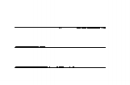
\includegraphics[width=0.5\columnwidth]{B10opt1.png}
    \caption*{}
    \label{fig:opt1}
\end{figure}
\item \begin{figure}[H]
    \centering
    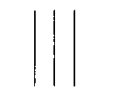
\includegraphics[width=0.5\columnwidth]{B10opt2.png}
    \caption*{}
    \label{fig:opt2}
\end{figure}
\item \begin{figure}[H]
    \centering
    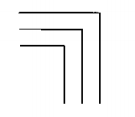
\includegraphics[width=0.5\columnwidth]{B10opt3.png}
    \caption*{}
    \label{fig:opt3}
\end{figure}
\item \begin{figure}[H]
    \centering
    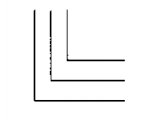
\includegraphics[width=0.5\columnwidth]{B10opt4.png}
    \caption*{}
    \label{fig:opt4}
\end{figure}
\end{enumerate}
\end{multicols}

\item A cricket ball comprises of a seam running along its central section, which is essentially stitching of two hemi-spheres. The seam creates additional roughness. The bowler releases the ball with seam orientation as shown in the figure below.
\begin{figure}[H]
    \centering
    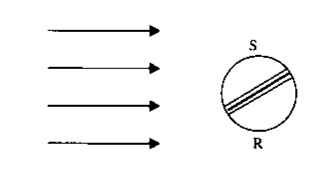
\includegraphics[width=0.3\columnwidth]{Bq11.png}
    \caption*{}
    \label{fig:q11}
\end{figure}
This would result in an out swinger with side forces on the cricket ball. These side forces on the ball are attributed to
\hfill{\brak{\text{GATE XE 2010}}}

\begin{enumerate}
\item flow having a laminar boundary layer separation on both sides.
\item flow having turbulent boundary layer separation on both sides.
\item flow having a laminar boundary layer separation on the side "S" and a turbulent boundary layer separation on the side "R".
\item flow having a laminar boundary layer separation on the side "R" and a turbulent boundary layer separation on the side "S".
\end{enumerate}

\item Ancients have designed water clocks based upon the head of the water in a circular section container with a hole at the bottom as shown in the figure below. The radius (r) varies as a function of head (H) to maintain a constant rate of decline of H.
\begin{figure}[H]
    \centering
    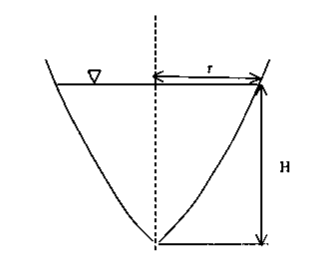
\includegraphics[width=0.4\columnwidth]{Bq12.png}
    \caption*{}
    \label{fig:q12}
\end{figure}
The relation between H and r is
\hfill{\brak{\text{GATE XE 2010}}}

\begin{multicols}{2}
\begin{enumerate}
\item H is proportional to r
\item H is proportional to $r^2$
\item H is proportional to $r^3$
\item H is proportional to $r^4$
\end{enumerate}
\end{multicols}

\item A 20 cm diameter pipe carries a water discharge of $\pi/100$ m$^3$/s. The pipe is bent through an angle of 30\degree in the horizontal plane as shown in the figure below.
\begin{figure}[H]
    \centering
    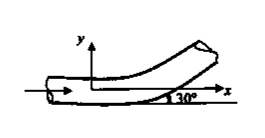
\includegraphics[width=0.4\columnwidth]{Bq13.png}
    \caption*{}
    \label{fig:q13}
\end{figure}
Neglecting friction, the components of the force (N) exerted by water on the bend in x- and y-directions, respectively, are
\hfill{\brak{\text{GATE XE 2010}}}

\begin{multicols}{2}
\begin{enumerate}
\item 4.21 and -15.71
\item -4.21 and 15.71
\item 15.71 and -27.2
\item 4.21 and 15.71
\end{enumerate}
\end{multicols}

\item A differential U-tube manometer with mercury as the manometric fluid is used to measure the pressure difference between two sections P and Q in a horizontal pipe carrying water at steady state as shown in the figure below. If the difference in mercury levels in the two limbs of the manometer is 0.75 m, the difference in pressure (kPa) between sections P and Q is
\begin{figure}[H]
    \centering
    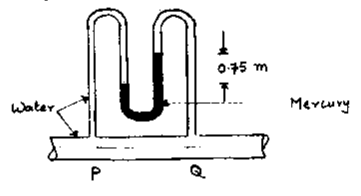
\includegraphics[width=0.4\columnwidth]{Bq14.png}
    \caption*{}
    \label{fig:q14}
\end{figure}
\hfill{\brak{\text{GATE XE 2010}}}

\begin{multicols}{4}
\begin{enumerate}
\item 49.275
\item 94.275
\item 9.4275
\item 492.75
\end{enumerate}
\end{multicols}

\item Two walls are holding back water as shown in the figures below. The resisting moments per unit length of the walls at points P and Q are $M_P$ and $M_Q$. Denoting the specific weight of water as $\gamma$, the difference in the moments ($M_Q - M_P$) is
\begin{figure}[H]
    \centering
    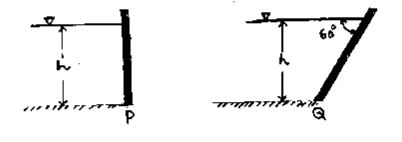
\includegraphics[width=0.6\columnwidth]{Bq15.png}
    \caption*{}
    \label{fig:q15}
\end{figure}
\hfill{\brak{\text{GATE XE 2010}}}

\begin{multicols}{2}
\begin{enumerate}
\item $\frac{\sqrt{3}\gamma h^3}{2}$
\item $\frac{2\gamma h^3}{\sqrt{3}}$
\item $\frac{\gamma h^3}{18}$
\item $\frac{\gamma h^3}{2}$
\end{enumerate}
\end{multicols}

\item A 20 cm cubical box slides on oil (mass density = 800 kg/m$^3$), over a large plane surface with a steady state velocity of 0.4 m/s. The plane surface is inclined at an angle of 30\degree with the horizontal plane. The oil film between the block and the plane surface is 0.4 mm thick. The weight of the cubical box is 64 N. The kinematic viscosity of the oil is
\hfill{\brak{\text{GATE XE 2010}}}

\begin{multicols}{2}
\begin{enumerate}
\item 0.8 Pa.s
\item 0.001 m$^2$/s
\item 1.6 Pa.s
\item 0.002 m$^2$/s
\end{enumerate}
\end{multicols}

\textbf{Common Data for Questions 17 and 18:} \\
A 60\% efficient pump is installed in a pipe of diameter 20 cm to lift water from a sump to an overhead tank at a discharge rate of $\pi/100$ m$^3$/s. Free surface level in the overhead tank is 20 m higher than the free surface level in the sump. The all-inclusive head losses \brak{\text{not including the lift}} in the suction and delivery sides of the pump are 2 times and 28 times the velocity head, respectively.

\item The power (\brak{\text{W}} supplied to the pump is
\hfill{\brak{\text{GATE XE 2010}}}

\begin{multicols}{4}
\begin{enumerate}
\item 10476.2
\item 6285.7
\item 6757.1
\item 11261.9
\end{enumerate}
\end{multicols}

\item The suction side of the pump is located L m above the free surface level in the sump. The minimum permissible pressure in the pipeline on the suction side of the pump is 8 m of water below atmospheric pressure. The maximum permissible value of L is
\hfill{\brak{\text{GATE XE 2010}}}

\begin{multicols}{4}
\begin{enumerate}
\item 20.00
\item 8.00
\item 7.85
\item 5.00
\end{enumerate}
\end{multicols}

\textbf{Common Data for Questions 19 and 20:} \\
The velocity field of a two-dimensional fluid flow is as follows:
\[ u = U_0 \frac{x}{L}, \quad v = -U_0 \frac{y}{L} \]
Where, $U_0$ and L are, respectively, the characteristic velocity and length.

\item If L = 0.2 m and the resultant of total accelerations in x- and y- directions at (x = L, y = L) is 10 m/s$^2$, the magnitude of $U_0$ (m/s) is
\hfill{\brak{\text{GATE XE 2010}}}

\begin{multicols}{4}
\begin{enumerate}
\item 1.414
\item 2.38
\item 1.19
\item 11.90
\end{enumerate}
\end{multicols}

\item The above fluid flow can be described as
\hfill{\brak{\text{GATE XE 2010}}}

\begin{multicols}{2}
\begin{enumerate}
\item rotational and compressible
\item irrotational and compressible
\item rotational and incompressible
\item irrotational and incompressible
\end{enumerate}
\end{multicols}

\textbf{Statement for Linked Answer Questions 21 and 22:} \\
The boundary layer formation over a flat plate is shown in the figure below. The variation of horizontal velocity (u) with y at any x along the plate in the boundary layer is approximated as: $u = P \sin(Qy) + R$
\begin{figure}[H]
    \centering
    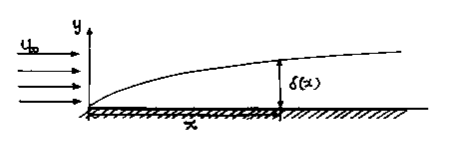
\includegraphics[width=0.6\columnwidth]{Bq21_22.png}
    \caption*{}
    \label{fig:q21_22}
\end{figure}

\item The most acceptable boundary conditions are
\hfill{\brak{\text{GATE XE 2010}}}

\begin{enumerate}
\item at y = 0, u = 0; at y = $\delta$, u = $U_\infty$; at y = 0, $\frac{du}{dy} = 0$
\item at y = 0, u = $U_\infty$; at y = $\delta$, u = $U_\infty$; at y = 0, $\frac{du}{dy} = 0$
\item at y = 0, u = 0; at y = $\delta$, u = $U_\infty$; at y = $\delta$, $\frac{du}{dy} = 0$
\item at y = 0, u = $U_\infty$; at y = $\delta$, u = $U_\infty$; at y = $\delta$, $\frac{du}{dy} = 0$
\end{enumerate}

\item Expressions for P, Q and R are
\hfill{\brak{\text{GATE XE 2010}}}

\begin{multicols}{2}
\begin{enumerate}
\item P = 0; Q = 0; R = 0
\item P = $U_\infty$; Q = 0; R = 0
\item P = 0; Q = $\frac{\pi}{2\delta}$; R = $U_\infty$
\item P = $U_\infty$; Q = $\frac{\pi}{2\delta}$; R = 0
\end{enumerate}
\end{multicols}
\end{enumerate}

\newpage

\section*{C: MATERIAL SCIENCE}

\begin{center}
    \textbf{Useful Data}
\end{center}
\begin{table}[H]
    \centering
    \begin{center}
    \begin{tabular}{|l l|}
        \hline
         Avogadro's number&:$6.023x10^{23}mol^{-1}$  \\
         Boltzmann's constant($k_B$)&:$1.38x10^{-23}$ \\
         Electron charge($e$)&:$1.602x10^{-19}$\\
         Gas Constant&:$8.314Jmol^{-1}K^{-1}$\\
         Electron rest mass&:$9.1x10^{-31}kg$\\
         Permittivity of vacuum($\epsilon_o$)&:$8.854x10^{-12}Fm^{-1}$\\
         Planck's constant($h$)&:$6.626x10^{-34}Js^{-1}$\\
         Bohr magneton($\mu_B$)&:$9.27x10^{-24}Am^{-2}$\\
         Free space permeability($\mu_o$)&:$4\pi 10^{-7}Hm^{-1}$\\
         $1J=6.242x10^{18}eV$&\\
         $1eV=1.602x10^{-19}J$&\\
         $1cal=4.2J$\\
         \hline
    \end{tabular}
\end{center}
    \caption*{}
    \label{useful_data}
\end{table}
\begin{enumerate}
\item The number of lattice points in an ideal Perovskite unit cell is
\hfill{\brak{\text{GATE XE 2010}}}

\begin{multicols}{4}
\begin{enumerate}
\item 1
\item 2
\item 4
\item 5
\end{enumerate}
\end{multicols}

\item A Frenkel defect is
\hfill{\brak{\text{GATE XE 2010}}}

\begin{enumerate}
\item a pair of cation and anion vacancy
\item a pair of cation interstitial and cation vacancy
\item a cation vacancy
\item an anion vacancy
\end{enumerate}

\item The angle between the line vector of a screw dislocation and the Burgers vector is
\hfill{\brak{\text{GATE XE 2010}}}

\begin{multicols}{4}
\begin{enumerate}
\item 0 degree
\item 45 degrees
\item 60 degrees
\item 90 degrees
\end{enumerate}
\end{multicols}

\item The addition of a network modifier to silica
\hfill{\brak{\text{GATE XE 2010}}}

\begin{enumerate}
\item produces vacancies
\item enhances the network structure
\item disrupts the network structure
\item increases the viscosity
\end{enumerate}

\item The best semiconductor material for LED in the visible range is
\hfill{\brak{\text{GATE XE 2010}}}

\begin{multicols}{4}
\begin{enumerate}
\item Si
\item Ge
\item GaAs
\item GaAs$_{0.6}$P$_{0.4}$
\end{enumerate}
\end{multicols}

\item A plain carbon steel sample is water- quenched from 900\degree C to room temperature. Its microstructure will consist of
\hfill{\brak{\text{GATE XE 2010}}}

\begin{multicols}{2}
\begin{enumerate}
\item pearlite
\item bainite
\item martensite
\item ferrite and pearlite
\end{enumerate}
\end{multicols}

\item Graphite at zero Kelvin is a
\hfill{\brak{\text{GATE XE 2010}}}

\begin{multicols}{4}
\begin{enumerate}
\item good conductor
\item insulator
\item semiconductor
\item semi-metal
\end{enumerate}
\end{multicols}

\item A high molecular weight polyethylene has an average molecular weight of 560,000g/mol. Its average degree of polymerization is
\hfill{\brak{\text{GATE XE 2010}}}

\begin{multicols}{4}
\begin{enumerate}
\item 15,000
\item 18,660
\item 19,310
\item 20,000
\end{enumerate}
\end{multicols}

\item In which region of the spectra crystal lattice absorption is very significant
\hfill{\brak{\text{GATE XE 2010}}}

\begin{multicols}{4}
\begin{enumerate}
\item ultraviolet
\item visible
\item microwave
\item infrared
\end{enumerate}
\end{multicols}

\item Match the properties in Column I with appropriate units in Column II
\begin{table}[H]
\centering
\begin{tabular}{ll}
\textbf{Column I} & \textbf{Column II} \\
P. viscosity & 1. m$^2$s$^{-1}$ \\
Q. diffusivity & 2. Kg mm$^2$ \\
R. charge mobility & 3. Nm$^{-2}$s \\
S. fracture toughness & 4. m$^2$V$^{-1}$s$^{-1}$ \\
 & 5. MPa$\sqrt{\text{m}}$ \\
\end{tabular}
\caption*{}
\label{tab:q10_mat}
\end{table}
\hfill{\brak{\text{GATE XE 2010}}}

\begin{multicols}{2}
\begin{enumerate}
\item P-3, Q-4, R-1, S-2
\item P-4, Q-1, R-2, S-5
\item P-5, Q-4, R-1, S-2
\item P-3, Q-1, R-4, S-5
\end{enumerate}
\end{multicols}

\item Match the terms in Column I with the details of phase transformations in Column II ($\rightarrow$ indicates cooling)
\begin{table}[H]
\centering
\begin{tabular}{ll}
\textbf{Column I} & \textbf{Column II} \\
P. eutectic & 1. L+ $\alpha \rightarrow \beta$ \\
Q. monotectic & 2. $\gamma \rightarrow \alpha + \beta$ \\
R. eutectoid & 3. L $\rightarrow \alpha + \beta$ \\
S. peritectic & 4. $\alpha + \beta \rightarrow \gamma$ \\
 & 5. L1 $\rightarrow \alpha$ + L2 \\
\end{tabular}
\caption*{}
\label{tab:q11_mat}
\end{table}
\hfill{\brak{\text{GATE XE 2010}}}

\begin{multicols}{2}
\begin{enumerate}
\item P-1, Q-5, R-4, S-3
\item P-3, Q-4, R-2, S-1
\item P-3, Q-5, R-2, S-1
\item P-5, Q-2, R-4, S-1
\end{enumerate}
\end{multicols}

\item Match the following materials in Column I with appropriate preparation technique given in Column II
\begin{table}[H]
\centering
\begin{tabular}{ll}
\textbf{Column I} & \textbf{Column II} \\
P. single crystals of laser materials & 1. sol-gel \\
Q. highly dense fine grained ceramics & 2. melt spinning \\
R. nanocrystalline oxide powders & 3. Bridgman-Stockbarger \\
S. metallic glasses & 4. hot pressing \\
 & 5. Czochralski \\
\end{tabular}
\caption*{}
\label{tab:q12_mat}
\end{table}
\hfill{\brak{\text{GATE XE 2010}}}

\begin{multicols}{2}
\begin{enumerate}
\item P-5, Q-4, R-1, S-2
\item P-3, Q-5, R-2, S-1
\item P-2, Q-1, R-4, S-5
\item P-5, Q-2, R-1, S-4
\end{enumerate}
\end{multicols}

\item Match the statement given in Column I with the most suitable material given in Column II
\begin{table}[H]
\centering
\begin{tabular}{ll}
\textbf{Column I} & \textbf{Column II} \\
P. biocompatible ceramic material & 1. zinc \\
Q. magnetic material with very high B-H product & 2. titanium \\
R. nonstick coating on aluminum & 3. Nd$_2$Fe$_{14}$B \\
S. sacrificial coating on steel & 4. Ca$_{10}$(PO$_4$)$_6$(OH)$_2$ \\
 & 5. BaFe$_{12}$O$_{19}$ \\
 & 6. polytetrafluoroethylene \\
 & 7. polyethylene terephthalate \\
\end{tabular}
\caption*{}
\label{tab:q13_mat}
\end{table}
\hfill{\brak{\text{GATE XE 2010}}}

\begin{multicols}{2}
\begin{enumerate}
\item P-4, Q-3, R-7, S-2
\item P-2, Q-5, R-6, S-1
\item P-4, Q-3, R-6, S-1
\item P-6, Q-5, R-7, S-6
\end{enumerate}
\end{multicols}

\item A 99\% pure copper wire has resistance of 0.1 $\Omega$ at 0.1 K, and 20 $\Omega$ at 300 K. For 100\% pure, perfect copper wire of the same size, the estimated resistance at 0.1 K and 300 K is
\hfill{\brak{\text{GATE XE 2010}}}

\begin{multicols}{2}
\begin{enumerate}
\item $\sim$ zero and 19.9 $\Omega$
\item $\sim$ zero and 20.1 $\Omega$
\item 0.1 and 19.9 $\Omega$
\item 0.1 and 20.1 $\Omega$
\end{enumerate}
\end{multicols}

\item A 12.0 mm diameter aluminum alloy test bar is subjected to a load of 110 kN. If the diameter of the bar is 10.5 mm at this load, the true strain will be
\hfill{\brak{\text{GATE XE 2010}}}

\begin{multicols}{4}
\begin{enumerate}
\item 0.134
\item 0.306
\item 0.267
\item 0.767
\end{enumerate}
\end{multicols}

\item If the effective magnetic moment of Fe$^{3+}$ is equal to 5 $\mu_B$, the magnetic moment in $\mu_B$ per formula of $\gamma$-Fe$_2$O$_3$ (which is inverse spinel with cation defects on the octahedral site) is
\hfill{\brak{\text{GATE XE 2010}}}

\begin{multicols}{4}
\begin{enumerate}
\item zero
\item 2.5
\item 5
\item 10
\end{enumerate}
\end{multicols}

\textbf{Common Data for Questions 17 and 18:} \\
A unidirectional carbon fiber epoxy matrix composite contains 60 vol \% carbon fibers. The density of carbon fiber is 1790 kg/m$^3$ and that of the epoxy matrix is 1200kg/m$^3$. The tensile moduli of the carbon fiber and the epoxy matrix are 340 GPa and 4.50 GPa respectively.

\item The density of the composite in the units of kg/m$^3$ is
\hfill{\brak{\text{GATE XE 2010}}}

\begin{multicols}{4}
\begin{enumerate}
\item 1495
\item 1554
\item 1672
\item 1790
\end{enumerate}
\end{multicols}

\item The tensile modulus of elasticity of the composite under iso-strain condition is
\hfill{\brak{\text{GATE XE 2010}}}

\begin{multicols}{4}
\begin{enumerate}
\item 5.5 GPa
\item 11.0 GPa
\item 102.9 GPa
\item 205.8 GPa
\end{enumerate}
\end{multicols}

\textbf{Common Data for questions 19 and 20:} \\
For a type II superconductor (at 4 K), the lower critical field (B$_{c1}$) and thermodynamic critical field (B$_c$) are respectively 0.001 Tesla and 0.10 Tesla.

\item The upper critical field (B$_{c2}$) in Tesla is
\hfill{\brak{\text{GATE XE 2010}}}

\begin{multicols}{4}
\begin{enumerate}
\item 0.10
\item 0.33
\item 1.00
\item 10.00
\end{enumerate}
\end{multicols}

\item The maximum energy that can be stored per unit volume (Jm$^{-3}$) in the superconductor is
\hfill{\brak{\text{GATE XE 2010}}}

\begin{multicols}{4}
\begin{enumerate}
\item $3.979 \times 10^3$
\item $50.00 \times 10^3$
\item $7.96 \times 10^3$
\item $1.326 \times 10^3$
\end{enumerate}
\end{multicols}

\textbf{Statement for linked Answer Questions 21 and 22:} \\
For Cu metal, the conduction electron density, n = $8.45 \times 10^{28}$ m$^{-3}$.

\item The energy of the electrons at the Fermi level (E$_F$) is
\hfill{\brak{\text{GATE XE 2010}}}

\begin{multicols}{4}
\begin{enumerate}
\item 3.50 eV
\item 7.028 eV
\item 8.45 eV
\item 49.0 eV
\end{enumerate}
\end{multicols}

\item The density of states (DOS), for 1cm$^3$ of Cu, at Fermi level per meV is
\hfill{\brak{\text{GATE XE 2010}}}

\begin{multicols}{4}
\begin{enumerate}
\item $1.20 \times 10^{19}$
\item $1.80 \times 10^{19}$
\item $1.20 \times 10^{22}$
\item $1.81 \times 10^{22}$
\end{enumerate}
\end{multicols}
\end{enumerate}

\section*{D: SOLID MECHANICS}
\begin{enumerate}
\item Three forces acting on a particle are given as
$\vec{F_1} = (5\hat{i}+6\hat{j})N$, $\vec{F_2} = (-\hat{i} +4\hat{k})N$ and $\vec{F_3} = (\hat{i}+6\hat{j}+16\hat{k})N$, where $\hat{i}, \hat{j}, \hat{k}$ are the unit vectors along Cartesian coordinate axes. Which one of the following statements is true?
\hfill{\brak{\text{GATE XE 2010}}}

\begin{enumerate}
\item Forces are coplanar and the particle is in equilibrium
\item Forces are coplanar but the particle is not in equilibrium
\item Forces are not coplanar but the particle is in equilibrium
\item Forces are not coplanar and the particle is not in equilibrium
\end{enumerate}

\item A truss consisting of members AD, DC, AB, BD and BC is subjected to a vertical force of 120 N at joint B as shown in the figure. The members AD, DC and BD are each of 1 meter length. The magnitude of force in the member BD is
\begin{figure}[H]
    \centering
    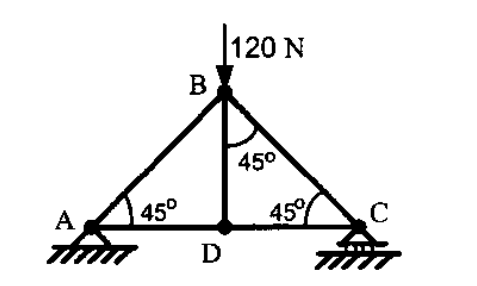
\includegraphics[width=0.4\columnwidth]{Dq2.png}
    \caption*{}
    \label{fig:q2_solid}
\end{figure}
\hfill{\brak{\text{GATE XE 2010}}}

\begin{multicols}{4}
\begin{enumerate}
\item 0
\item $20\sqrt{2}$ N
\item 40 N
\item 120 N
\end{enumerate}
\end{multicols}

\item Two rigid bodies A and B are each weighing 30 N. Body A is kept on a floor and body B is kept on body A as shown in the figure. The coefficient of friction between two bodies, and between body A and the floor is 0.1. If a horizontal force of 2 N is applied on body A, the friction force at the interface of body A and body B will be
\begin{figure}[H]
    \centering
    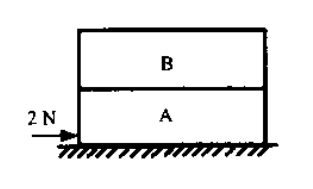
\includegraphics[width=0.3\columnwidth]{Dq3.png}
    \caption*{}
    \label{fig:q3_solid}
\end{figure}
\hfill{\brak{\text{GATE XE 2010}}}

\begin{multicols}{4}
\begin{enumerate}
\item 0
\item 1 N
\item 2 N
\item 3 N
\end{enumerate}
\end{multicols}

\item A rigid link PQ is rotating about a revolute joint at P with a uniform angular velocity $\omega$. A slider R is sliding on the link with a relative velocity v. Which one of the following figures represents the correct direction of the Coriolis acceleration $a_c$?
\hfill{\brak{\text{GATE XE 2010}}}

\begin{multicols}{2}
\begin{enumerate}
\item \begin{figure}[H]
    \centering
    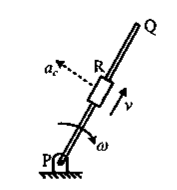
\includegraphics[width=0.5\columnwidth]{D4opt1.png}
    \caption*{}
    \label{fig:opt1}
\end{figure}
\item \begin{figure}[H]
    \centering
    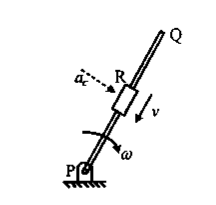
\includegraphics[width=0.5\columnwidth]{D4opt2.png}
    \caption*{}
    \label{fig:opt2}
\end{figure}
\item \begin{figure}[H]
    \centering
    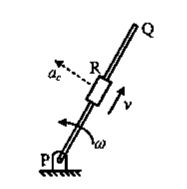
\includegraphics[width=0.5\columnwidth]{D4opt3.png}
    \caption*{}
    \label{fig:opt3}
\end{figure}
\item \begin{figure}[H]
    \centering
    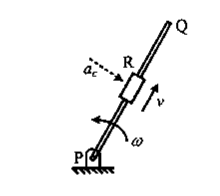
\includegraphics[width=0.5\columnwidth]{D4opt4.png}
    \caption*{}
    \label{fig:opt4}
\end{figure}
\end{enumerate}
\end{multicols}

\item A bullet of mass m having a horizontal velocity of 500 m/s hits a stationary block of mass 6.15 kg. The block breaks into two parts viz. Q \brak{\text{mass of 3 kg}} and R \brak{\text{mass of 3.15 kg}}, with the bullet embedded in R. The parts Q and R travel in the direction of initial velocity of the bullet. If the velocity of Q is 3 m/s and the velocity of R is 5 m/s, the mass of the bullet m is
\hfill{\brak{\text{GATE XE 2010}}}

\begin{multicols}{4}
\begin{enumerate}
\item 5 kg
\item 0.5 kg
\item 0.05 kg
\item 0.005 kg
\end{enumerate}
\end{multicols}

\item Two particles, P and Q, are initially at two ends of a circular arc which subtends an angle of 120\degree at the arc-center. The radius of the arc is r. The particles P and Q are moving along the arc towards each other with constant tangential velocities of $v_P$ and $v_Q$ respectively. The distance travelled by the particle P when it meets the particle Q is
\hfill{\brak{\text{GATE XE 2010}}}

\begin{multicols}{2}
\begin{enumerate}
\item $\frac{2\pi r}{3} \frac{(v_P + v_Q)}{v_P}$
\item $\frac{2\pi r}{3} \frac{(v_P + v_Q)}{v_Q}$
\item $\frac{2\pi}{3} \frac{r v_P}{(v_P + v_Q)}$
\item $\frac{2\pi}{3} \frac{r v_Q}{(v_P + v_Q)}$
\end{enumerate}
\end{multicols}

\item Which one of the following plane states of stress corresponds to Mohr's circle of radius zero?
\hfill{\brak{\text{GATE XE 2010}}}

\begin{figure}[H]
    \centering
    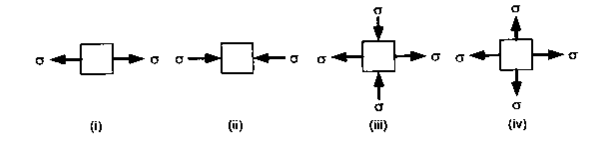
\includegraphics[width=0.8\columnwidth]{Dq7.png}
    \caption*{}
    \label{fig:q7_solid}
\end{figure}

\item Maximum shear stress theory for material yielding is known as
\hfill{\brak{\text{GATE XE 2010}}}

\begin{multicols}{2}
\begin{enumerate}
\item Tresca's criterion
\item von-Mises criterion
\item Saint-Venant's theory
\item Rankine's theory
\end{enumerate}
\end{multicols}

\item In a cantilever beam of length 2 m, the shear force in newton \brak{\text{N}} along the length is given by $V(x) = 5x^2$, where x is the distance in meter measured from the fixed end. The magnitude of the load intensity at the mid-span of the beam is
\hfill{\brak{\text{GATE XE 2010}}}

\begin{multicols}{4}
\begin{enumerate}
\item 0
\item 1 N/m
\item 5 N/m
\item 10 N/m
\end{enumerate}
\end{multicols}

\item Two blocks P and Q are connected by a string, which passes over a pulley as shown in the figure. The block P is sliding on an inclined surface. Ignoring the masses of the string and the pulley, the tension in the string is \brak{\text{use gravitational acceleration g = 9.81 m/s$^2$ and neglect all friction}}
\begin{figure}[H]
    \centering
    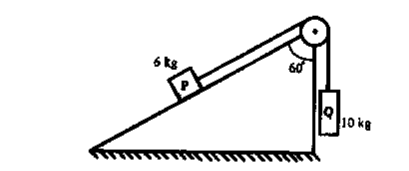
\includegraphics[width=0.4\columnwidth]{Dq10.png}
    \caption*{}
    \label{fig:q10_solid}
\end{figure}
\hfill{\brak{\text{GATE XE 2010}}}

\begin{multicols}{4}
\begin{enumerate}
\item 55.2 N
\item 62.5 N
\item 74.3 N
\item 86.2 N
\end{enumerate}
\end{multicols}

\item A hollow circular shaft of inside diameter 10 mm and outside diameter 20 mm is subjected to a pure symmetric-bending moment of 200 N-m. The magnitude of bending stress at a point in the plane of loading, which is at a distance of 5 mm from the neutral axis, is
\hfill{\brak{\text{GATE XE 2010}}}

\begin{multicols}{4}
\begin{enumerate}
\item 0
\item 68.8 MPa
\item 135.8 MPa
\item 271.6 MPa
\end{enumerate}
\end{multicols}

\item A stepped circular shaft made of steel is rigidly fixed at two supports A and C as shown in the figure. A torque of 680 N-m is applied on the shaft at point B. The diameter of portion AB is twice that of portion BC. The magnitudes of torque reactions at supports A and C respectively are
\begin{figure}[H]
    \centering
    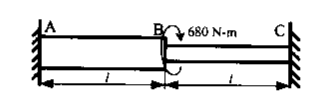
\includegraphics[width=0.6\columnwidth]{Dq12.png}
    \caption*{}
    \label{fig:q12_solid}
\end{figure}
\hfill{\brak{\text{GATE XE 2010}}}

\begin{multicols}{2}
\begin{enumerate}
\item 640 N-m, 40 N-m
\item 40 N-m, 640 N-m
\item 340 N-m, 340 N-m
\item 544 N-m, 136 N-m
\end{enumerate}
\end{multicols}

\item A thin-walled cylinder with open ends is subjected to uniform internal pressure p alone. The wall thickness is t, internal radius is r and the Young's modulus is E. The increase in radius of the cylinder due to the internal pressure is
\hfill{\brak{\text{GATE XE 2010}}}

\begin{multicols}{2}
\begin{enumerate}
\item zero
\item $\frac{pr^2}{2Et}$
\item $\frac{pr^2}{Et}$
\item $\frac{pr}{Et} + r$
\end{enumerate}
\end{multicols}

\item A cylindrical steel bar of uniform cross-sectional area is subjected to an axial tensile force P and a torque T. Assuming linear elastic deformation of the bar, the internal strain energy stored in the bar is $(20P^2 + 8T^2) \times 10^{-6}$ N-m. The axial extension of the bar for P = 10 N and T = 16 N-m is
\hfill{\brak{\text{GATE XE 2010}}}

\begin{multicols}{4}
\begin{enumerate}
\item 256 $\mu$m
\item 400 $\mu$m
\item 2000 $\mu$m
\item 2048 $\mu$m
\end{enumerate}
\end{multicols}

\item The buckling load of a slender column clamped at both the ends is 4000 N. The column is subjected to an axial compression. During the course of service, one of the ends gets detached from the clamp and becomes free end. The absolute percentage change in the buckling load due to the change in the end condition is
\hfill{\brak{\text{GATE XE 2010}}}

\begin{multicols}{4}
\begin{enumerate}
\item 50.00
\item 75.00
\item 83.25
\item 93.75
\end{enumerate}
\end{multicols}

\item A spring-mass system shown in the figure is vibrating with very small amplitude. The natural frequency of the system is
\begin{figure}[H]
    \centering
    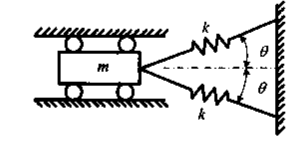
\includegraphics[width=0.4\columnwidth]{Dq16.png}
    \caption*{}
    \label{fig:q16_solid}
\end{figure}
\hfill{\brak{\text{GATE XE 2010}}}

\begin{multicols}{4}
\begin{enumerate}
\item $\sqrt{\frac{k}{m}}$
\item $\sqrt{\frac{2k}{m}}$
\item $\sqrt{\frac{2k \cos \theta}{m}}$
\item $\sqrt{\frac{2k \cos^2 \theta}{m}}$
\end{enumerate}
\end{multicols}

\textbf{Common Data for Questions 17 and 18:} \\
Two particles P and Q are connected by a rigid link of negligible mass. The length of the link PQ is $\sqrt{2} r$. The inner radius of the ring is r and its centre is at O as shown in the figure. The particles are allowed to slide freely with negligible friction on the inner surface of a vertical circular ring. The angle $\theta$, between OQ and horizontal X-axis, is measured from X-axis in the clockwise sense. Gravitational acceleration is g.
\begin{figure}[H]
    \centering
    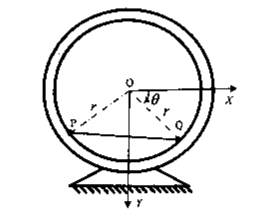
\includegraphics[width=0.4\columnwidth]{Dq17_18.png}
    \caption*{}
    \label{fig:q17_18_solid}
\end{figure}

\item Mass of the particles P and Q are m and 2m, respectively. The link PQ is released from $\theta = 0^\circ$. When the link occupies the horizontal position, the magnitude of velocity of particle P is
\hfill{\brak{\text{GATE XE 2010}}}

\begin{multicols}{4}
\begin{enumerate}
\item $0.865\sqrt{gr}$
\item $1.865\sqrt{gr}$
\item $0.086\sqrt{gr}$
\item $2.865\sqrt{gr}$
\end{enumerate}
\end{multicols}

\item If both the particles P and Q are of the mass m and the link PQ is released from $\theta = 0^\circ$, the maximum possible value of $\theta$ during the oscillation of the link is
\hfill{\brak{\text{GATE XE 2010}}}

\begin{multicols}{4}
\begin{enumerate}
\item 45$^\circ$
\item 90$^\circ$
\item 135$^\circ$
\item 180$^\circ$
\end{enumerate}
\end{multicols}

\textbf{Common Data for Questions 19 and 20:} \\
A cantilever beam of length 3l is subjected to two forces each of magnitude P as shown in the figure. The flexural rigidity of the beam is EI. Assume linear elastic material and small deflections.
\begin{figure}[H]
    \centering
    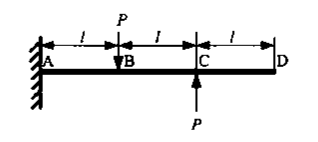
\includegraphics[width=0.6\columnwidth]{Dq19_20.png}
    \caption*{}
    \label{fig:q19_20_solid}
\end{figure}

\item Which one of the following statements is true?
\hfill{\brak{\text{GATE XE 2010}}}

\begin{enumerate}
\item The magnitude of the bending moment in portion AB is zero
\item The magnitude of the bending moment in portion AB is Pl
\item The magnitude of the bending moment in portion AB is 2Pl
\item The magnitude of the bending moment in portion AB varies linearly from 0 to Pl
\end{enumerate}

\item The deflection due to bending at point B is
\hfill{\brak{\text{GATE XE 2010}}}

\begin{multicols}{2}
\begin{enumerate}
\item $\frac{Pl^3}{3EI} \downarrow \brak{\text{downward}}$
\item $\frac{Pl^3}{2EI} \uparrow \brak{\text{upward}}$
\item $\frac{Pl^3}{6EI} \downarrow \brak{\text{downward}}$
\item $\frac{Pl^3}{6EI} \uparrow \brak{\text{upward}}$
\end{enumerate}
\end{multicols}

\textbf{Statement for Linked Answer Questions 21 and 22:} \\
A steel bar of rectangular cross-section is heated uniformly and the rise in the temperature is $\Delta T$. The Young's modulus is E, the Poisson's ratio is $\nu$ and the coefficient of thermal expansion is $\alpha$. The bar is completely restrained in the axial direction and lateral directions.

\item The thermal stress developed in the bar along the axial direction is
\hfill{\brak{\text{GATE XE 2010}}}

\begin{multicols}{2}
\begin{enumerate}
\item $\frac{E\alpha\Delta T}{1+2\nu}$
\item $-E\alpha\Delta T$
\item $-\frac{E\alpha\Delta T}{1-2\nu}$
\item $\frac{E\alpha\Delta T \nu}{1-2\nu}$
\end{enumerate}
\end{multicols}

\item Assume that the bar is allowed to deform freely in the lateral directions, while keeping the axial direction restrained. The percentage change in the magnitude of axial thermal stress for $\nu = 0.25$ is
\hfill{\brak{\text{GATE XE 2010}}}

\begin{multicols}{4}
\begin{enumerate}
\item 0
\item 25
\item 50
\item 100
\end{enumerate}
\end{multicols}
\end{enumerate}

\section*{E: THERMODYNAMICS}
\begin{enumerate}
\item Match the items in Group I for their correctness with the corresponding appropriate terms given in Groups II and III.
\begin{table}[H]
\centering
\begin{tabular}{lll}
\textbf{GROUP I} & \textbf{GROUP II} & \textbf{GROUP III} \\
P: Pressure & 1: Path dependent quantity & X: Intensive property \\
Q: Heat & 2: Path independent quantity & Y: Extensive property \\
\end{tabular}
\caption*{}
\label{tab:q1_thermo}
\end{table}
\hfill{\brak{\text{GATE XE 2010}}}

\begin{multicols}{4}
\begin{enumerate}
\item P,1,X
\item P,2,X
\item Q,1,X
\item Q,2,Y
\end{enumerate}
\end{multicols}

\item An object of mass 'm' in a wooden box having mass 'M' falls through a height 'h' under the influence of gravity in vacuum. The work done by the object on the box is
\begin{flushright}
\brak{\text{GATE XE 2010}}
\end{flushright}

\begin{multicols}{4}
\begin{enumerate}
\item 0
\item mgh
\item Mgh
\item (m+M)gh
\end{enumerate}
\end{multicols}

\item An ideal gas is known to obey following relationships: $u = 200 + 0.718T$ and $Pv = 0.287(T + 273)$, where u is specific internal energy \brak{\text{kJ/kg}}, T is temperature \brak{\text{\degree C}}, P is pressure \brak{\text{kPa}} and v is specific volume \brak{\text{m$^3$/kg}}. Specific heat \brak{\text{in kJ/kg-K}} at constant pressure is
\hfill{\brak{\text{GATE XE 2010}}}

\begin{multicols}{4}
\begin{enumerate}
\item 0.287
\item 0.431
\item 0.718
\item 1.005
\end{enumerate}
\end{multicols}

\item A heat pump, which operates in a cycle, extracts heat energy from the cold reservoir and supplies the same amount of energy to the hot reservoir. Which of the following statements holds for this process?
\hfill{\brak{\text{GATE XE 2010}}}

\begin{enumerate}
\item This process violates both the first and the second law
\item This process violates the first law but not the second law
\item This process violates the second law but not the first law
\item This process does not violate both first and second law
\end{enumerate}

\item An insulated rigid container having 1 m$^3$ volume has two compartments having equal volume separated by a thin membrane. Half of the container is filled with helium \brak{\text{R = 2.08 kJ/kg-K, $C_p = 5.19$ kJ/kg-K and $C_v = 3.11$ kJ/kg-K}}, while the remaining half is empty. Suddenly the membrane ruptures and helium fills the whole volume of the container. Temperature and pressure of helium before rupture are 500\degree C and 0.1 MPa respectively. The change in the entropy of helium is
\hfill{\brak{\text{GATE XE 2010}}}

\begin{multicols}{4}
\begin{enumerate}
\item 0.019 kJ/K
\item 0.045 kJ/K
\item 0.112 kJ/K
\item 0.675 kJ/K
\end{enumerate}
\end{multicols}

\item 1 kg of methane is enclosed in a cylinder having volume 6.4 litres and is maintained at a temperature of 13\degree C and pressure of 18.56 MPa. If molecular weight of methane is 16 kg/kmol \brak{\text{for methane, critical pressure = 4.64 MPa, critical temperature is 191.1 K; universal gas constant is 8.314 kJ/kmol-K}}, compressibility factor, Z, is
\begin{flushright}
\brak{\text{GATE XE 2010}}
\end{flushright}

\begin{multicols}{4}
\begin{enumerate}
\item 0.375
\item 0.8
\item 1.25
\item 2.66
\end{enumerate}
\end{multicols}

\item $\brak{\frac{\partial P}{\partial T}}_v$ is equal to
\hfill{\brak{\text{GATE XE 2010}}}

\begin{multicols}{2}
\begin{enumerate}
\item $\brak{\frac{\partial s}{\partial v}}_P$
\item $-\brak{\frac{\partial s}{\partial v}}_T$
\item $\brak{\frac{\partial s}{\partial v}}_T$
\item $-\brak{\frac{\partial s}{\partial v}}_P$
\end{enumerate}
\end{multicols}

\item A rigid spherical vessel contains 1 kg of wet steam of quality x at pressure $P_1$. This is shown by point A on the T-v diagram. Heat is transferred to the vessel to form superheated steam at pressure $P_2$ and temperature $T_2$, as shown by point B.
\begin{figure}[H]
    \centering
    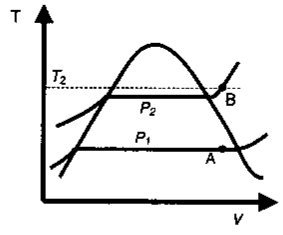
\includegraphics[width=0.4\columnwidth]{Eq8.png}
    \caption*{}
    \label{fig:q8_thermo}
\end{figure}
Specific enthalpy and specific internal energy corresponding to the saturated water and saturated vapour at pressures $P_1$ and $P_2$ as well as at points A and B are given by
\begin{table}[H]
\centering
\caption*{}
\label{tab:q8_thermo}
\begin{tabular}{|l|c|c|c|c|c|c|}
\hline
 & \multicolumn{2}{c|}{Saturated liquid} & \multicolumn{2}{c|}{Saturated vapour} & Point & Point \\
\cline{2-5}
Property & Pressure $P_1$ & Pressure $P_2$ & Pressure $P_1$ & Pressure $P_2$ & A & B \\
\hline
Specific Enthalpy & $h_{f1}$ & $h_{f2}$ & $h_{g1}$ & $h_{g2}$ & $h_A$ & $h_B$ \\
\brak{\text{kJ/kg}} & & & & & & \\
\hline
Specific internal & $u_{f1}$ & $u_{f2}$ & $u_{g1}$ & $u_{g2}$ & $u_A$ & $u_B$ \\
energy \brak{\text{kJ/kg}} & & & & & & \\
\hline
\end{tabular}
\end{table}
Heat transferred to the steam is
\hfill{\brak{\text{GATE XE 2010}}}

\begin{multicols}{2}
\begin{enumerate}
\item $h_B - h_A$
\item $h_B - h_{f1}$
\item $u_B - u_A$
\item $u_B - u_{f1}$
\end{enumerate}
\end{multicols}

\item Determine the correctness or otherwise of the following Assertion [a] and the Reason [r] \\
\textbf{Assertion:} Carnot cycle is not used in vapour power cycles. \\
\textbf{Reason:} Pumping of a two phase mixture is difficult
\hfill{\brak{\text{GATE XE 2010}}}

\begin{enumerate}
\item Both [a] and [r] are true and [r] is a reason for [a]
\item Both [a] and [r] are true but [r] is NOT a reason for [a]
\item [a] is true but [r] is false
\item Both [a] and [r] are false
\end{enumerate}

\item A slab of mass 2000 kg and volume 0.2 m$^3$ is raised slowly in the vertical direction by a massless rope through a height of 2 m from the bottom of a fresh-water lake. Depth of water in the lake is 10 m. If the density of fresh water is 1000 kg/m$^3$ and acceleration due to gravity is 10 m/s$^2$, work done by water on the block is
\hfill{\brak{\text{GATE XE 2010}}}

\begin{multicols}{4}
\begin{enumerate}
\item -40 kJ
\item 0 kJ
\item 4 kJ
\item +40 kJ
\end{enumerate}
\end{multicols}

\item A bulb is connected to a U-tube with long vertical column as shown in the figure below. Cross-sectional area of both sides of the U-tube is 1 cm$^3$. Water is poured in the right side open column of the U-tube such that the trapped air in the left column and the bulb above water has a volume of 1000 cc and a pressure of 105 kPa. Ambient pressure is 100 kPa. Density of water is 1000 kg/m$^3$. Acceleration due to gravity may be taken as 10 m/s$^2$.
\begin{figure}[H]
    \centering
    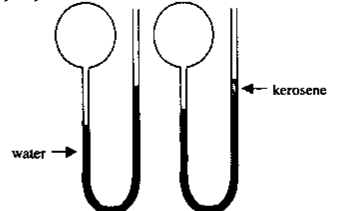
\includegraphics[width=0.6\columnwidth]{Eq11.png}
    \caption*{}
    \label{fig:q11_thermo}
\end{figure}
When 90 cc of kerosene oil \brak{\text{specific gravity = 0.7}} is poured on the right side of the U-tube, water level in the left column rises by 10 cm. The pressure in the bulb becomes
\hfill{\brak{\text{GATE XE 2010}}}

\begin{multicols}{4}
\begin{enumerate}
\item 105.1 kPa
\item 108.3 kPa
\item 112.4 kPa
\item 119.7 kPa
\end{enumerate}
\end{multicols}

\item Air \brak{\text{R=287 J/kg-K, $C_p$=1005 J/kg-K and $\gamma$=1.4}} flows sequentially through a compressor, a heater and a turbine as shown in the figure. Volume flow rate of air coming out from the compressor is 2.33m$^3$/s when pressure and temperature are 276 kPa and 43 \degree C respectively. Air is then heated at same pressure to 430 \degree C in a heater. From heater, air flows through a turbine which produces 1860 kW of power. Heat loss from turbine to the surrounding is 90 kW. Air temperature at the turbine exit is
\begin{figure}[H]
    \centering
    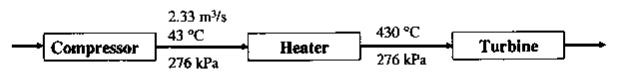
\includegraphics[width=1\columnwidth]{Eq12.png}
    \caption*{}
    \label{fig:q12_thermo}
\end{figure}
\hfill{\brak{\text{GATE XE 2010}}}

\begin{multicols}{4}
\begin{enumerate}
\item 156.4\degree C
\item 181.6\degree C
\item 223.7\degree C
\item 678.4\degree C
\end{enumerate}
\end{multicols}

\item Availability per unit mass associated with air \brak{\text{R = 287 J/kg-K, $C_p$ = 1005 J/kg-K and $\gamma$ = 1.4}} flowing from a reservoir at 10 atm and 25\degree C when atmosphere is at 1 atm and 25\degree C is \brak{\text{Neglect changes in the potential and the kinetic energies}}
\hfill{\brak{\text{GATE XE 2010}}}

\begin{multicols}{4}
\begin{enumerate}
\item 98.4 kJ/kg
\item 196.9 kJ/kg
\item 492.3 kJ/kg
\item 689.14 kJ/kg
\end{enumerate}
\end{multicols}

\item In an air standard Diesel cycle, compression ratio is 14. At the beginning of compression of air \brak{\text{R = 287 J/kg-K, $C_p$ = 1005 J/kg-K and $\gamma$ = 1.4}} the temperature is 27\degree C and the pressure is 1 bar. If the specific volume after heat addition is two times the specific volume after compression, heat added \brak{\text{in kJ per kg of air}} at constant pressure is
\hfill{\brak{\text{GATE XE 2010}}}

\begin{multicols}{4}
\begin{enumerate}
\item 555.5
\item 622.7
\item 767.8
\item 866.4
\end{enumerate}
\end{multicols}

\item A mixture of Freon and air is supplied for cleaning a chamber. The mixture contains 70\% by volume of air and 30\% by volume of Freon. Specific heat ratios for Freon and air are 1.1 and 1.4 respectively. Molecular mass of Freon is 200 g/mole and that of air is 30 g/mole. Temperature of gas is 300 K. If, universal gas constant is 8.314 J/mole-K, specific heat ratio of the mixture is
\hfill{\brak{\text{GATE XE 2010}}}

\begin{multicols}{4}
\begin{enumerate}
\item 1.16
\item 1.21
\item 1.25
\item 1.31
\end{enumerate}
\end{multicols}

\item Air-water vapour mixture having 100\% relative humidity at 50\degree C is heated isobarically to 100\degree C in a closed system. If saturation pressure at 50\degree C is 12.352 kPa and at 100\degree C is 101.42 kPa, final relative humidity is
\hfill{\brak{\text{GATE XE 2010}}}

\begin{multicols}{4}
\begin{enumerate}
\item 0\%
\item 8.2\%
\item 12.2\%
\item 100\%
\end{enumerate}
\end{multicols}

\textbf{Common Data for Questions 17 and 18:} \\
Saturated vapour enters a turbine at a pressure of 2 bar and leaves the turbine at a pressure of 0.1 bar and a quality of 0.9. After condensation, saturated water at 0.1 bar is pumped into the boiler where it receives heat at a constant pressure of 2 bar. The pumping process can be considered to be isentropic. Use the data given in the following table to answer Q17 and Q18.
\begin{table}[H]
\centering
\caption*{}
\label{tab:q17_18_thermo}
\begin{tabular}{|c|c|cc|cc|cc|}
\hline
Pressure & Saturation & \multicolumn{2}{c|}{Specific volume} & \multicolumn{2}{c|}{Specific enthalpy} & \multicolumn{2}{c|}{Specific entropy} \\
\brak{\text{bar}} & temperature \brak{\text{\degree C}} & \multicolumn{2}{c|}{(m$^3$/kg)} & \multicolumn{2}{c|}{(kJ/kg)} & \multicolumn{2}{c|}{(kJ/kg-K)} \\
\hline
 & & $v_f$ & $v_g$ & $h_f$ & $h_g$ & $s_f$ & $s_g$ \\
2 & 120.23 & 0.001061 & 0.8857 & 504.68 & 2706.6 & 1.530 & 7.1271 \\
0.1 & 45.81 & 0.001010 & 14.674 & 191.81 & 2584.6 & 0.6492 & 8.1501 \\
\hline
\end{tabular}
\end{table}

\item Work done by the turbine is
\hfill{\brak{\text{GATE XE 2010}}}

\begin{multicols}{4}
\begin{enumerate}
\item 276.5 kJ/kg
\item 303.9 kJ/kg
\item 335.8 kJ/kg
\item 361.3 kJ/kg
\end{enumerate}
\end{multicols}

\item Heat addition in the boiler is
\hfill{\brak{\text{GATE XE 2010}}}

\begin{multicols}{4}
\begin{enumerate}
\item 2000.9 kJ/kg
\item 2514.6 kJ/kg
\item 3028.2 kJ/kg
\item 3554.5 kJ/kg
\end{enumerate}
\end{multicols}

\textbf{Common Data for Questions 19 and 20:} \\
An insulated piston-cylinder assembly having a paddle wheel, as shown in the adjacent figure, contains air \brak{\text{R = 287 J/kg-K, and $C_v$ = 718 J/kg-K}} of mass 4 kg. Both piston and paddle wheel can be considered as insulated and massless. Temperature and pressure of air inside the cylinder are 300 K and 100 kPa respectively. Ambient pressure is 100 kPa.
\begin{figure}[H]
    \centering
    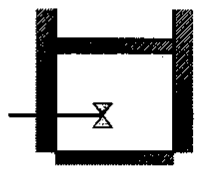
\includegraphics[width=0.3\columnwidth]{Eq19_20.png}
    \caption*{}
    \label{fig:q19_20_thermo}
\end{figure}

\item If the piston is locked in the fixed position and the paddle wheel delivers 75 kJ of work, final air temperature is
\hfill{\brak{\text{GATE XE 2010}}}

\begin{multicols}{4}
\begin{enumerate}
\item 300 K
\item 318.7 K
\item 320.6 K
\item 326.1 K
\end{enumerate}
\end{multicols}

\item If the piston is free to slide without any friction when the paddle wheel delivers 75 kJ of work, final temperature of air in the cylinder is
\hfill{\brak{\text{GATE XE 2010}}}

\begin{multicols}{4}
\begin{enumerate}
\item 305.2 K
\item 309.3 K
\item 312.6 K
\item 318.7 K
\end{enumerate}
\end{multicols}

\textbf{Statement for Linked Answer Questions 21 and 22:} \\
In a process industry, two different streams of water \brak{\text{to be considered incompressible}} are available at 10\degree C and 90\degree C as shown in the figure. Mass flow rates of both the streams are 1 kg/s. Rather than wasting these resources, it is desired to connect a reversible Carnot engine that will continuously extract heat from the hot stream and supply part of it to the cold stream such that the exit temperature of both the streams $T_f$, is identical. Heat capacity of water is 4.18 kJ/kg-K.
\begin{figure}[H]
    \centering
    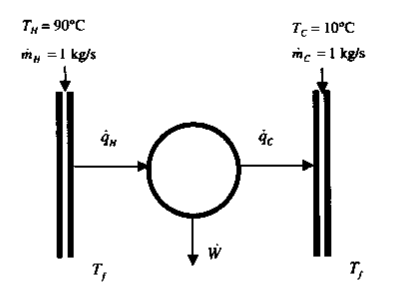
\includegraphics[width=0.6\columnwidth]{Eq21_22.png}
    \caption*{}
    \label{fig:q21_22_thermo}
\end{figure}

\item Value of $T_f$ is
\hfill{\brak{\text{GATE XE 2010}}}

\begin{multicols}{4}
\begin{enumerate}
\item 30 \degree C
\item 42.5 \degree C
\item 47.5 \degree C
\item 50 \degree C
\end{enumerate}
\end{multicols}

\item Work output $\dot{W}$ is:
\hfill{\brak{\text{GATE XE 2010}}}

\begin{multicols}{4}
\begin{enumerate}
\item 20.8 kW
\item 42.5 kW
\item 63 kW
\item 167 kW
\end{enumerate}
\end{multicols}
\end{enumerate}

\section*{F: POLYMER SCIENCE AND ENGINEERING}
\begin{enumerate}
\item Which one of the following molecules undergoes ring opening polymerization?
\begin{flushright}
\brak{\text{GATE XE 2010}}
\end{flushright}

\begin{multicols}{2}
\begin{enumerate}
\item \begin{figure}[H]
    \centering
    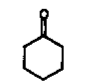
\includegraphics[width=0.5\columnwidth]{F1opt1.png}
    \caption*{}
    \label{fig:opt1}
\end{figure}
\item \begin{figure}[H]
    \centering
    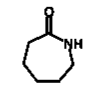
\includegraphics[width=0.5\columnwidth]{F1opt2.png}
    \caption*{}
    \label{fig:opt2}
\end{figure}
\item \begin{figure}[H]
    \centering
    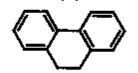
\includegraphics[width=0.5\columnwidth]{F1opt3.png}
    \caption*{}
    \label{fig:opt3}
\end{figure}
\item \begin{figure}[H]
    \centering
    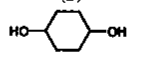
\includegraphics[width=0.5\columnwidth]{F1opt4.png}
    \caption*{}
    \label{fig:opt4}
\end{figure}
\end{enumerate}
\end{multicols}

\item Out of the following polymers, which one shows the highest melting temperature?
\begin{flushright}
\brak{\text{GATE XE 2010}}
\end{flushright}

\begin{enumerate}
\item Poly\brak{\text{ethylene terephthalate}}
\item Poly\brak{\text{propylene terephthalate}}
\item Poly\brak{\text{butylene terephthalate}}
\item Poly\brak{\text{hexylene terephthalate}}
\end{enumerate}

\item Which one of the following reagents is used to prevent coagulation of natural rubber latex?
\hfill{\brak{\text{GATE XE 2010}}}

\begin{multicols}{2}
\begin{enumerate}
\item Ammonia
\item Acetic acid
\item Tolyl mercaptan
\item Sodium chloride
\end{enumerate}
\end{multicols}

\item From the following four groups of polymers, identify the group in which all four polymers are semicrystalline
\hfill{\brak{\text{GATE XE 2010}}}

\begin{multicols}{2}
\begin{enumerate}
\item HDPE, PP, PS, UF
\item PET, PVC, PF, ABS
\item Nylon 6, EPDM, PMMA, SBR
\item Nylon 66, PP, HDPE, PET
\end{enumerate}
\end{multicols}

\item If $\eta$ represents viscosity of polymer solution and $\eta_0$ represents viscosity of pure solvent, then the specific viscosity ($\eta_{sp}$) of the polymer solution is expressed as
\begin{flushright}
\brak{\text{GATE XE 2010}}
\end{flushright}

\begin{multicols}{4}
\begin{enumerate}
\item $\frac{\eta}{\eta_0}$
\item $\frac{\eta}{\eta_0} - 1$
\item $\frac{\eta_0-1}{\eta}$
\item $\frac{\eta_0}{\eta}$
\end{enumerate}
\end{multicols}

\item A polymer blend is developed by mixing
\hfill{\brak{\text{GATE XE 2010}}}

\begin{multicols}{2}
\begin{enumerate}
\item A polymer and a monomer
\item A polymer and a stabilizer
\item A polymer with another polymer
\item A polymer and a filler
\end{enumerate}
\end{multicols}

\item In shear deformation of a polymer melt, the unit of shear rate is
\hfill{\brak{\text{GATE XE 2010}}}

\begin{multicols}{4}
\begin{enumerate}
\item m$^2$sec$^{-1}$
\item m$^2$sec$^{-1}$
\item msec$^{-1}$
\item sec$^{-1}$
\end{enumerate}
\end{multicols}

\item A rubber compound is made by mixing functional additives with the rubber using
\begin{flushright}
\brak{\text{GATE XE 2010}}
\end{flushright}

\begin{multicols}{2}
\begin{enumerate}
\item Two-roll mill
\item Compression molding machine
\item Three-roll calender
\item Thermoforming machine
\end{enumerate}
\end{multicols}

\item The group of polymers consisting of LDPE, PP, PS and PVC is best categorized as
\begin{flushright}
\brak{\text{GATE XE 2010}}
\end{flushright}

\begin{multicols}{2}
\begin{enumerate}
\item Engineering polymers
\item Biodegradable polymers
\item Commodity polymers
\item Natural polymers
\end{enumerate}
\end{multicols}

\item A small molecule is eliminated as a byproduct during the synthesis of
\hfill{\brak{\text{GATE XE 2010}}}

\begin{multicols}{2}
\begin{enumerate}
\item Polycaprolactone
\item Poly(ethylene terephthalate)
\item Styrene butadiene copolymer
\item Polytetrafluoroethylene
\end{enumerate}
\end{multicols}

\item For free radical copolymerization of monomers $M_1$ and $M_2$, if the reactivity ratios $r_1$ and $r_2$ are both found to be zero, then the resulting copolymer is
\hfill{\brak{\text{GATE XE 2010}}}

\begin{multicols}{2}
\begin{enumerate}
\item Random
\item Branched
\item Block
\item Alternating
\end{enumerate}
\end{multicols}

\item Pair each item in Column I with the appropriate one in Column II
\begin{table}[H]
\centering
\begin{tabular}{ll}
\textbf{Column I} & \textbf{Column II} \\
P. Shampoo bottles & 1. Injection molding \\
Q. Overhead tank & 2. Extrusion \\
R. Helmet & 3. Blow molding \\
S. Insulation for cables & 4. Rotomolding \\
\end{tabular}
\caption*{}
\label{tab:q12_poly}
\end{table}
\hfill{\brak{\text{GATE XE 2010}}}

\begin{multicols}{2}
\begin{enumerate}
\item P-1; Q-2; R-4; S-3
\item P-2; Q-1; R-3; S-4
\item P-3; Q-4; R-1; S-2
\item P-4; Q-3; R-2; S-1
\end{enumerate}
\end{multicols}

\item Toughness of a plastic material can be judged from the area under the stress-strain curve obtained from tensile test. The plastic having the highest toughness exhibits
\hfill{\brak{\text{GATE XE 2010}}}

\begin{multicols}{2}
\begin{enumerate}
\item High tensile strength and low elongation
\item Low tensile strength and high elongation
\item High tensile strength and high elongation
\item Low tensile strength and low elongation
\end{enumerate}
\end{multicols}

\item Match the following additives for plastics with their respective functions
\begin{table}[H]
\centering
\begin{tabular}{ll}
\textbf{Additives} & \textbf{Functions} \\
P. Iron oxide & 1. Blowing agent \\
Q. Azodicarbonamide & 2. Coloring agent \\
R. Phenyl salicylate & 3. Filler \\
S. Calcium carbonate & 4. UV stabilizer \\
\end{tabular}
\caption*{}
\label{tab:q14_poly}
\end{table}
\hfill{\brak{\text{GATE XE 2010}}}

\begin{multicols}{2}
\begin{enumerate}
\item P-1; Q-2; R-3; S-4
\item P-2; Q-1; R-4; S-3
\item P-3; Q-4; R-1; S-2
\item P-4; Q-3; R-2; S-1
\end{enumerate}
\end{multicols}

\item The volume fraction of epoxy resin in a glass fibre/epoxy composite is 0.48. The densities of glass fibre and composite are 2540 kg/m$^3$ and 1950 kg/m$^3$, respectively. The weight fraction of the fibre in the composite is
\hfill{\brak{\text{GATE XE 2010}}}

\begin{multicols}{4}
\begin{enumerate}
\item 0.68
\item 0.52
\item 0.48
\item 0.32
\end{enumerate}
\end{multicols}

\item The change of shear stress with shear rate of a polymer melt as shown in the figure below indicates
\begin{figure}[H]
    \centering
    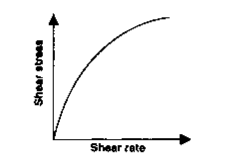
\includegraphics[width=0.4\columnwidth]{Fq16.png}
    \caption*{}
    \label{fig:q16_poly}
\end{figure}
\hfill{\brak{\text{GATE XE 2010}}}
\begin{enumerate}
\item Viscosity increase with increase in shear rate
\item Viscosity decrease with increase in shear rate
\item Viscosity remaining independent of shear rate
\item Viscosity oscillation with increase in shear rate
\end{enumerate}

\textbf{Common Data for Questions 17 and 18:} \\
For polyesterification of HO-\brak{\text{CH$_2$}}$_{14}$-COOH, the number average degree of polymerization, $\bar{X}_n$, is related to the stoichiometric imbalance $r$ between the functional groups and the extent of polymerization $p$ by the equation
\[ \bar{X}_n = \frac{1+r}{1+r-2rp} \]

\item For 100\% polyesterification, the $\bar{X}_n$ will be
\hfill{\brak{\text{GATE XE 2010}}}

\begin{multicols}{4}
\begin{enumerate}
\item 100
\item 1000
\item 10000
\item $\infty$
\end{enumerate}
\end{multicols}

\item The percentage conversion of functional groups required to obtain the polyester with a molecular weight of 24000 g/mol will be
\hfill{\brak{\text{GATE XE 2010}}}

\begin{multicols}{4}
\begin{enumerate}
\item 99
\item 96
\item 93
\item 90
\end{enumerate}
\end{multicols}

\textbf{Common Data for Questions 19 and 20:} \\
The glass transition temperatures of PVC, plasticized PVC and nitrile rubber are 81 \degree C, -3 \degree C and -50 \degree C, respectively. For making a plastic raincoat, 40 mass percent of polymeric plasticizer is added to PVC.

\item The glass transition temperature of the polymeric plasticizer will be
\hfill{\brak{\text{GATE XE 2010}}}

\begin{multicols}{4}
\begin{enumerate}
\item -84 \degree C
\item -74 \degree C
\item 74 \degree C
\item 84 \degree C
\end{enumerate}
\end{multicols}

\item If the polymeric plasticizer is replaced by nitrile rubber to make the same raincoat, the mass percent of rubber to be blended with PVC is
\hfill{\brak{\text{GATE XE 2010}}}

\begin{multicols}{4}
\begin{enumerate}
\item 40
\item 47
\item 53
\item 60
\end{enumerate}
\end{multicols}

\textbf{Statement for Linked Answer Questions 21 and 22:} \\
A polydisperse polymer consists of the following three different fractions
\begin{table}[H]
\centering
\begin{tabular}{lccc}
 & Fraction I & Fraction II & Fraction III \\
Mass of polymer (\%) & 30 & 20 & 50 \\
Molecular weight (g/mol) & 30,000 & 80,000 & 150,000 \\
\end{tabular}
\caption*{}
\label{tab:q21_22_poly}
\end{table}

\item The number average molecular weight, $\bar{M}_n$ (g/mol) of the polymer is
\hfill{\brak{\text{GATE XE 2010}}}

\begin{multicols}{2}
\begin{enumerate}
\item $1.02 \times 10^5$
\item $0.99 \times 10^5$
\item $0.63 \times 10^5$
\item $0.55 \times 10^5$
\end{enumerate}
\end{multicols}

\item The polydispersity index of the polymer is
\hfill{\brak{\text{GATE XE 2010}}}

\begin{multicols}{4}
\begin{enumerate}
\item 2.59
\item 1.87
\item 1.72
\item 1.59
\end{enumerate}
\end{multicols}
\end{enumerate}

\section*{G: FOOD TECHNOLOGY}
\begin{enumerate}
\item A food material contains 70\% moisture (wet basis). The food is dried for 3 hours at 80\degree C air temperature in a tray dryer such that 80\% of its initial moisture is removed. Final moisture content (wet basis) of the dried food is
\hfill{\brak{\text{GATE XE 2010}}}

\begin{multicols}{4}
\begin{enumerate}
\item 31.82\%
\item 46.67\%
\item 56.00\%
\item 20.01\%
\end{enumerate}
\end{multicols}

\item Liquid A obeys power law equation $\sigma = k\dot{\gamma}^n$ (as shown in the attached figure) where $\sigma$ is shear stress, $\dot{\gamma}$ is shear rate, k is consistency index and n is flow behavior index.
\begin{figure}[H]
    \centering
    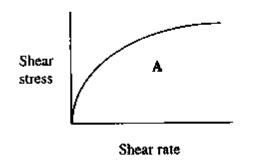
\includegraphics[width=0.4\columnwidth]{Gq2.png}
    \caption*{}
    \label{fig:q2_food}
\end{figure}
The correct unit of consistency index and nature of liquid are
\hfill{\brak{\text{GATE XE 2010}}}

\begin{multicols}{2}
\begin{enumerate}
\item Pa s and Shear thinning
\item Pa s$^n$ and Shear thickening
\item Pa s and Shear thickening
\item Pa s$^n$ and Shear thinning
\end{enumerate}
\end{multicols}

\item Identify the amino acid tyrosine from the following structures
\hfill{\brak{\text{GATE XE 2010}}}

\begin{multicols}{2}
\begin{enumerate}
\item \begin{figure}[H]
    \centering
    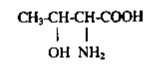
\includegraphics[width=0.8\columnwidth]{G3opt1.png}
    \caption*{}
    \label{fig:opt1}
\end{figure}
\item \begin{figure}[H]
    \centering
    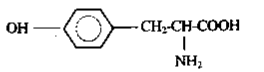
\includegraphics[width=0.8\columnwidth]{G3opt2.png}
    \caption*{}
    \label{fig:opt2}
\end{figure}
\item \begin{figure}[H]
    \centering
    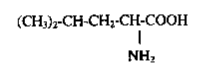
\includegraphics[width=0.8\columnwidth]{G3opt3.png}
    \caption*{}
    \label{fig:opt3}
\end{figure}
\item \begin{figure}[H]
    \centering
    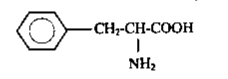
\includegraphics[width=0.8\columnwidth]{G3opt4.png}
    \caption*{}
    \label{fig:opt4}
\end{figure}
\end{enumerate}
\end{multicols}

\item Saponification number of a fat is the milligrams of KOH required to saponify 1 g of fat. The correct statement on saponification is
\hfill{\brak{\text{GATE XE 2010}}}

\begin{enumerate}
\item Fat with high amount of low molecular weight fatty acids will have high saponification number
\item Butter has low saponification number
\item Fatty acids with long carbon chains have high saponification number
\item Fat with low Reichert-Meissl number has very high saponification number
\end{enumerate}

\item The expansion of the terms HACCP and GRAS are
\hfill{\brak{\text{GATE XE 2010}}}

\begin{enumerate}
\item Hygienic Associated Critical Control Point; Grossly Recommended As Safe
\item Hazard Analysis and Critical Control Point; Generally Recognized As Safe
\item Hygienic and Aesthetic Concept of Critical Products; Generally Recognized As Safe
\item Hazard Analysis and Critical Control Point; Grossly Recommended As Safe
\end{enumerate}

\item Which two of the following statements are NOT the objectives of homogenization of milk? \\
i. Counteracting segregation for the most part of creaming thus avoiding sedimentation or phase separation \\
ii. Arresting rancidity of fat globules in milk \\
iii. Increasing fluidity of milk by lowering viscosity \\
iv. Improving the colour of the milk (more whitish) \\
v. Improving milk stability by preventing partial coalescence of fat globules
\hfill{\brak{\text{GATE XE 2010}}}

\begin{multicols}{4}
\begin{enumerate}
\item i and ii
\item ii and iii
\item iii and iv
\item iv and v
\end{enumerate}
\end{multicols}

\item Shelf-life of fish can be extended by chilling as it
\hfill{\brak{\text{GATE XE 2010}}}

\begin{enumerate}
\item reduces chemical activity of food constituents and increases biochemical activity
\item reduces water activity and increases biochemical reaction rate
\item reduces chemical and biochemical reactions in fish cells
\item destroys pathogenic microbes
\end{enumerate}

\item Major spoilage organisms of poultry meat at low temperatures are
\hfill{\brak{\text{GATE XE 2010}}}

\begin{multicols}{2}
\begin{enumerate}
\item Candida and Staphylococcus
\item Torula and Clostridium
\item Pseudomonas and Acinetobacter
\item Flavobacteria and Lactobacillus
\end{enumerate}
\end{multicols}

\item The appropriate explanation for spoilage of egg, stored at low temperature, might be due to:
\hfill{\brak{\text{GATE XE 2010}}}

\begin{enumerate}
\item Shell of egg is porous and only fungal hyphae can enter and contaminate the egg liquid
\item Shells are non-porous and the spoilage is mainly attributed to chemical decomposition
\item Shell of egg is porous and microorganisms contaminating the shell penetrate it and cause the spoilage
\item Eggs are contaminated before they are laid by hen
\end{enumerate}

\item Two faces of a metal plate having thermal conductivity 17 W m$^{-1}$ K$^{-1}$ and thickness 10 mm are maintained at 80\degree C and 100\degree C. If the thickness of the plate is increased by 20\% and the temperature of the hotter face is increased to 120\degree C, then the percent increase in heat flux under steady state heat transfer is
\hfill{\brak{\text{GATE XE 2010}}}

\begin{multicols}{4}
\begin{enumerate}
\item 20.67
\item 40.00
\item 59.99
\item 66.67
\end{enumerate}
\end{multicols}

\item Match the items in Group I with the most appropriate items in Group II
\begin{table}[H]
\centering
\begin{tabular}{ll}
\textbf{Group I} & \textbf{Group II} \\
P. Freeze concentration & 1. Triple point of water \\
Q. Reverse osmosis & 2. Heat transfer by conduction \\
R. Drum drying & 3. Eutectic point \\
S. Freeze drying & 4. Radiation heat transfer \\
 & 5. Concentration polarization \\
\end{tabular}
\caption*{}
\label{tab:q11_food}
\end{table}
\hfill{\brak{\text{GATE XE 2010}}}

\begin{multicols}{2}
\begin{enumerate}
\item P-4, Q-5, R-2, S-1
\item P-3, Q-2, R-5, S-1
\item P-3, Q-5, R-2, S-1
\item P-1, Q-2, R-4, S-3
\end{enumerate}
\end{multicols}

\item Match the following items in Group I and Group II in relation to nutritional requirement of human body
\begin{table}[H]
\centering
\begin{tabular}{ll}
\textbf{Group I} & \textbf{Group II} \\
P. Calcium and Phosphorus & 1. Elements not needed in diet \\
Q. Vitamin D & 2. Promotes absorption of iron \\
R. Manganese and Chromium & 3. Elements that are required in small quantities \\
S. Vitamin K & 4. Promotes the absorption of Calcium \\
 & 5. Essential for normal clotting of blood \\
 & 6. Elements that are required in large quantities \\
\end{tabular}
\caption*{}
\label{tab:q12_food}
\end{table}
\hfill{\brak{\text{GATE XE 2010}}}

\begin{multicols}{2}
\begin{enumerate}
\item P-6, Q-2, R-1, S-5
\item P-5, Q-2, R-6, S-4
\item P-6, Q-4, R-3, S-5
\item P-2, Q-5, R-1, S-4
\end{enumerate}
\end{multicols}

\item 9.5 g of corn flakes containing 5\% moisture (wet basis) is oxidized completely to CO$_2$ and H$_2$O by ignition in a Bomb Calorimeter (as shown in the figure). The combustion increases the temperature of 2500 g of water from 15\degree C to 27\degree C. Assume that the heat capacity and latent heat of vaporization of water are 4.187 kJ kg$^{-1}$ K$^{-1}$ and 2257 kJ kg$^{-1}$, respectively. Neglect any sensible heat gain by water vapour. The calorific value of the flake is
\begin{figure}[H]
    \centering
    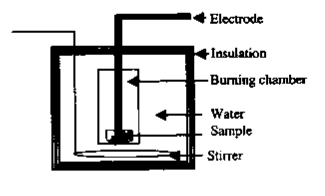
\includegraphics[width=0.8\columnwidth]{Gq13.png}
    \caption*{}
    \label{fig:q13_food}
\end{figure}
\hfill{\brak{\text{GATE XE 2010}}}

\begin{multicols}{2}
\begin{enumerate}
\item 18.28 kJ g$^{-1}$ (4.37 kcal g$^{-1}$)
\item 9.79 kJ g$^{-1}$ (2.34 kcal g$^{-1}$)
\item 14.04 kJ g$^{-1}$ (3.36 kcal g$^{-1}$)
\item 22.43 kJ g$^{-1}$ (5.36 kcal g$^{-1}$)
\end{enumerate}
\end{multicols}

\item Match the following items in Group I and Group II in relation to permitted food additives/preservatives in India
\begin{table}[H]
\centering
\begin{tabular}{ll}
\textbf{Group I} & \textbf{Group II} \\
P. Jelly & 1. Calcium propionate \\
Q. Edible oil & 2. Monosodium glutamate \\
R. Meat flavour enhancer & 3. Sodium benzoate \\
S. Bread & 4. Butylated hydroxylated anisole \\
 & 5. Tricalcium silicate \\
\end{tabular}
\caption*{}
\label{tab:q14_food}
\end{table}
\hfill{\brak{\text{GATE XE 2010}}}

\begin{multicols}{2}
\begin{enumerate}
\item P-3, Q-4, R-2, S-1
\item P-5, Q-3, R-2, S-4
\item P-1, Q-3, R-4, S-5
\item P-2, Q-3, R-1, S-5
\end{enumerate}
\end{multicols}

\item Preparation of sweet coated breakfast cereals like corn flakes includes several major processing steps, like \\
P: Soaking in water followed by steaming of corn grits \\
Q: Coating of sugar followed by drying of flakes \\
R: Breaking the whole corn into large grits \\
S: Flaking of cooked grits \\
T: Packaging of finished product \\
U: Toasting of flakes \\
V: Cleaning of whole corn \\
The correct sequence for the preparation of sugar coated corn flake is
\hfill{\brak{\text{GATE XE 2010}}}

\begin{enumerate}
\item V $\rightarrow$ U $\rightarrow$ Q $\rightarrow$ P $\rightarrow$ S $\rightarrow$ R $\rightarrow$ T
\item V $\rightarrow$ R $\rightarrow$ S $\rightarrow$ P $\rightarrow$ U $\rightarrow$ Q $\rightarrow$ T
\item V $\rightarrow$ U $\rightarrow$ P $\rightarrow$ Q $\rightarrow$ S $\rightarrow$ R $\rightarrow$ T
\item V $\rightarrow$ R $\rightarrow$ P $\rightarrow$ S $\rightarrow$ U $\rightarrow$ Q $\rightarrow$ T
\end{enumerate}

\item A bacterial strain isolated from meat is inoculated in a growth medium at a cell density of $2 \times 10^5$ cells/ml. Then, 0.2 ml of the culture broth is withdrawn immediately and mixed with 0.8 ml of sterile saline. This sample is diluted by mixing 0.1 ml of it with 99.9 ml sterile water. Then 0.1 ml of this diluted solution is spread on appropriate nutrient agar plate. The number of colonies expected on the agar plate is
\hfill{\brak{\text{GATE XE 2010}}}

\begin{multicols}{4}
\begin{enumerate}
\item 4
\item 40
\item 400
\item 4000
\end{enumerate}
\end{multicols}

\textbf{Common Data for Questions 17 and 18:} \\
Water at 20\degree C is pumped from a base tank to an elevated tank, 15 m above the base tank. Water flows at a rate of $5.0 \times 10^{-3}$ m$^3$ s$^{-1}$ through a pipe having internal diameter of 0.1023 m. Frictional energy loss in the pipe is 6.837 J kg$^{-1}$. The pump has an efficiency of 65\%. Density and viscosity of water are 998.2 kg m$^{-3}$ and $1.005 \times 10^{-3}$ Pa s, respectively.

\item Reynolds number for water flowing through the pipe is
\hfill{\brak{\text{GATE XE 2010}}}

\begin{multicols}{2}
\begin{enumerate}
\item $5.286 \times 10^4$
\item $6.180 \times 10^4$
\item $2.285 \times 10^4$
\item $1.252 \times 10^4$
\end{enumerate}
\end{multicols}

\item Power needed for pumping water in kW is
\hfill{\brak{\text{GATE XE 2010}}}

\begin{multicols}{4}
\begin{enumerate}
\item 1.182
\item 3.334
\item 0.985
\item 2.226
\end{enumerate}
\end{multicols}

\textbf{Common Data for Questions 19 and 20:} \\
True density and bulk density of rice grain are 1230 kg m$^{-3}$ and 740 kg m$^{-3}$, respectively, and that of wheat grain are 1360 kg m$^{-3}$ and 650 kg m$^{-3}$, respectively.

\item The void fractions of a bed of rice and that of wheat are respectively.
\hfill{\brak{\text{GATE XE 2010}}}

\begin{multicols}{4}
\begin{enumerate}
\item 0.331 and 0.546
\item 0.662 and 0.261
\item 0.398 and 0.480
\item 0.398 and 0.522
\end{enumerate}
\end{multicols}

\item Assume the bulk volume for the mixture of two grains follows additive rule. If the bulk density of a mixture of rice and wheat is 700 kg m$^{-3}$, weight percentage of wheat in the mixture is nearly
\hfill{\brak{\text{GATE XE 2010}}}

\begin{multicols}{4}
\begin{enumerate}
\item 41
\item 50
\item 24
\item 36
\end{enumerate}
\end{multicols}

\textbf{Statement for Linked Answer Questions 21 and 22:} \\
D$_T$ value of a bacterium is determined by using two thin walled glass capillary tubes filled with same bacterial suspension in distilled water. The sealed capillaries are dipped in an oil bath maintained at 121\degree C and kept for 60 s and 135 s, respectively. These capillaries are cooled immediately in ice water. Number of survivals remained in the respective tubes are 2000 and 300.

\item D$_T$ value (in minutes) of the bacterium is
\hfill{\brak{\text{GATE XE 2010}}}

\begin{multicols}{4}
\begin{enumerate}
\item 1.32
\item 0.52
\item 1.52
\item 2.52
\end{enumerate}
\end{multicols}

\item The processing time (in minutes) to kill 99.999\% of the bacteria in any food at 121\degree C will be
\hfill{\brak{\text{GATE XE 2010}}}

\begin{multicols}{4}
\begin{enumerate}
\item 7.60
\item 6.60
\item 12.62
\item 2.60
\end{enumerate}
\end{multicols}
\end{enumerate}

\end{document}
